\documentclass{article}
\usepackage{graphicx}
\usepackage{amsmath}
\usepackage{amssymb}
\usepackage[a4paper, top=25mm, bottom=25mm, left=25mm, right=25mm]{geometry}
\usepackage{pgfplots}
\pgfplotsset{compat=1.18}

\begin{document}
\large

\begin{center}
2016-2017 Fall Semester\\MAT123-07 Midterm\\(05.12.2016)
\end{center}

\noindent 1) Evaluate the following limits.

\hfill

\noindent a) $\displaystyle \lim_{x \to \infty} [\mathrm{e}^x + 1]^{\frac{1}{x}}$

\hfill

\noindent b) $\displaystyle \lim_{x \to 1} \frac{x-1}{\sqrt{x+3} - 2}$

\hfill

\noindent 2) For which values of $a$ is

\[
f(x) =
\begin{cases}
a^2x - 2a, & x \geq 2 \\
12,  & x < 2
\end{cases}
\]

\noindent continuous at every $x$?

\hfill

\noindent 3) Find an equation for the tangent line to the curve $ y = x^{\sin x}$, at the point $(\frac{\pi}{2}, \frac{\pi}{2})$.

\hfill

\noindent 4) The length of a rectangle decreases at 3 cm/s, while its width increases at 2 cm/s. At a certain moment, the rectangle is 50 cm long and 20 cm wide. Is the area of the rectangle increasing or decreasing, and how fast?

\hfill

\noindent 5) Sketch the graph of $\displaystyle y = \frac{2x^2}{x^2-1}$.

\hfill

\noindent 6) Show that the equation $x^4 + 3x + 1$ has exactly one solution in the interval $[-2, -1]$.

\newpage

\begin{center}
Solutions (Last update: 07/10/25 (10th of July) 8:52 PM)
\end{center}

\noindent 1)

\hfill

\noindent a) To solve the limit easily, we can use logarithms. The expression is continuous and differentiable for $x > 0$. Assume that the limit exists, then let L be the value of the limit.

\begin{equation*} L = \lim_{x \to \infty} [\mathrm{e}^x + 1]^{\frac{1}{x}} \end{equation*}

\begin{equation*}
\ln(L) = \ln\Big(\lim_{x \to \infty} [\mathrm{e}^x + 1]^{\frac{1}{x}}\Big) = \lim_{x \to \infty} \Big[ \ln\Big( [\mathrm{e}^x + 1]^{\frac{1}{x}} \Big) \Big]
\end{equation*}

\begin{equation*}
\ln(L) = \lim_{x \to \infty} \Big[ \frac{\ln(\mathrm{e}^x + 1)}{x}\Big]
\end{equation*}

\hfill

\noindent The expressions $x$ and $\mathrm{e}^x + 1$ tend to infinity as $x$ approaches infinity. L'Hôpital's rule suggests that we take the derivatives of both sides of the fraction if there's an indeterminate form of infinity ($\frac{\infty}{\infty}$). Using the chain rule, we get:

\begin{equation*}
\ln(L) \overset{\text{L'H.}}{=} \lim_{x \to \infty} \Big[ \frac{\frac{1}{\mathrm{e}^x+1} \cdot \mathrm{e}^x}{1} \Big] = \lim_{x \to \infty} \Big( \frac{\mathrm{e}^x}{\mathrm{e}^x+1} \Big)
\end{equation*}

\hfill

\noindent It is obvious that $\ln(L) = 1$. $\mathrm{e}^x$ grows at the same rate as $\mathrm{e}^x + 1$. The behavior can be confirmed using L'Hôpital's rule. Without further ado, we can convert the logarithm back to its original form.

\begin{equation*}\ln(L) = 1\end{equation*}
\begin{equation*}\boxed{L = \mathrm{e}}\end{equation*}

\hfill

\noindent b) If we substitute for $x = 1$, it is in the form $0/0$. Multiply each side by the conjugate of the denominator.

\begin{equation*}
\lim_{x \to 1}\Big( \frac{x-1}{\sqrt{x+3} - 2} \cdot \frac{\sqrt{x+3} + 2}{\sqrt{x+3} + 2} \Big) = \lim_{x \to 1} \frac{(x-1)(\sqrt{x+3} + 2)}{x-1} = \lim_{x \to 1} (\sqrt{x+3} + 2) = \boxed 4\end{equation*}

\hfill

\noindent 2) If $f$ is continuous at a point, then the one-sided limits must be equal to the value of the function at that point. $f$ is constant for $x < 2$, meanwhile polynomial for $x \geq 2$. If we check the point where $x=2$, the continuity will be provided for all $x$.

\begin{equation*}\lim_{x \to 2^-} f(x) = 12,\, \lim_{x \to 2^+} f(x) = a^2x-2a \,\rightarrow\, 12 = 2a^2-2a \end{equation*}

\begin{equation*} 2(a^2-a - 6) = 0\,\rightarrow\,(a-3)(a+2) = 0\,\rightarrow\,\boxed{a_1 = 3,\,a_2 = -2}\end{equation*}

\hfill

\noindent 3) Take logarithms of both sides. Then differentiate implicitly.

\begin{equation*}y(x) = x^{\sin x}\end{equation*}
\begin{equation*}\ln(y) = \sin x \cdot \ln x\end{equation*}

\begin{equation*}\frac{d}{dx}\ln(y) = \frac{d}{dx}(\sin x \cdot \ln x)\end{equation*}

\begin{equation*} \frac{1}{y} \cdot \frac{dy}{dx} =  \cos x \cdot \ln x +  \sin x \cdot \frac{1}{x}\end{equation*}

\begin{equation} \frac{dy}{dx} = x^{\sin x}\Big(\cos x \cdot \ln x +  \sin x \cdot \frac{1}{x}\Big)\end{equation}

\hfill

\noindent Recall: $y-y_0 = m(x-x_0)$, where $m$ is the slope. We can evaluate $(1)$ at $x = \frac{\pi}{2}$ because $\frac{dy}{dx}|_{(\pi/2,\, \pi/2)}$ gives the rate of change at that point.

\[x_0 = \frac{\pi}{2},\,y_0 = \frac{\pi}{2}\]

\[m = \frac{dy}{dx}\Bigg|_{(\pi/2,\, \pi/2)} = \Big(\frac{\pi}{2}\Big)^{\sin \frac{\pi}{2}}\Big(\cos\frac{\pi}{2} \cdot \ln \frac{\pi}{2} + \sin \frac{\pi}{2} \cdot \frac{2}{\pi}\Big) = 1\]

\hfill

\noindent Therefore, the tangent line is $\boxed{y=x}$.

\hfill

\noindent 4) Let $w$, $l$ be the functions of time representing width and length, respectively, Then the area of the rectangle can be written as:

\begin{equation*}
A(t) = w(t)\cdot l(t)
\end{equation*}

\hfill

\noindent Take the derivative of both sides with respect to $t$. Apply the chain rule.

\begin{equation*}\frac{d}{dt}A(t) = \frac{d}{dt}(w(t)\cdot l(t))\end{equation*}

\begin{equation*}A'(t) = w'(t)\cdot l(t) + w(t)\cdot l'(t)\end{equation*}

\hfill

\noindent Let $t_1$ be the moment when as told in the question.

\begin{equation*}l'(t_1) = -3,\,\,w'(t_1) = 2,\,\,l(t_1) = 50,\,\, w(t_1) = 20\end{equation*}

\begin{equation*}A'(t_1) = 2\cdot 50 - 20\cdot 3 = 40\end{equation*}

\begin{equation*}\boxed{A'(t_1) = 40\, \text{cm}^2/\text{s}}\end{equation*}

\hfill

\noindent Since $A'(t_1) > 0$, the area increases at $t=t_1$.

\hfill

\noindent 5) First off, find the domain. The expression is undefined when the denominator is zero. Therefore, $x^2-1 \neq 0 \,\rightarrow\, x\neq \pm 1$. Vertical asymptotes occur at $x = \pm 1$.

\begin{equation*}\text{D} = \mathbb{R} - \{-1, 1\} \end{equation*}

\hfill

\noindent Let us find the limit at infinity.

\begin{equation*}\lim_{x\to \infty} \frac{2x^2}{x^2-1} \overset{\text{L'H.}}{=} \lim_{x\to \infty} \frac{4x}{2x} = \lim_{x\to \infty} 2 = 2\end{equation*}

\noindent Similarly,

\begin{equation*}\lim_{x\to -\infty} \frac{2x^2}{x^2-1} = 2\end{equation*}

\hfill

\noindent $y=2$ is the only horizontal asymptote. Now, let us glance at the critical points. This will give us an idea of where the graph becomes stationary. Take the first derivative. Apply the quotient rule.

\begin{equation*}\frac{d}{dx}(y) = \frac{d}{dx}\Big(\frac{2x^2}{x^2-1}\Big)\end{equation*}

\begin{equation*}y' = \frac{4x\cdot(x^2-1) - 2x^2 \cdot 2x}{(x^2-1)^2} = -\frac{4x}{(x^2-1)^2} \end{equation*}

\hfill

\noindent For $x=0$, $y'=0$. (0,0) is a critical point. Look for the inflection points now. Take the second derivative.

\begin{equation*}y'' = -\frac{4\cdot (x^2-1)^2 - 4x \cdot 2(x^2-1)(2x)}{(x^2-1)^4} = \frac{12x^2+4}{(x^2-1)^3} \end{equation*}

\hfill

\noindent $\forall x \in \mathbb{R},\,12x^2+4 > 0$. Therefore, no inflection points.

\hfill

\noindent Eventually, set up a table and see what the graph looks like in certain intervals.

\begin{center}
    \large
    \begin{tabular}{ |c| c c c c| } 
    \hline
        $x$ & $(-\infty, -1)$ & $(-1, 0)$ & $(0, 1)$ &  $(1, \infty)$ \\
        \hline
        $y$ & $(2, \infty)$ & $(-\infty, 0]$ & $(-\infty, 0]$ & $[2, \infty]$\\
        \hline
        $y'$ sign & + & + & - & - \\
        \hline
        $y''$ sign & + & - & - & + \\
        \hline
    \end{tabular}
\end{center}

\hfill

\noindent Knowing that $f(0) = 0$, we may sketch the graph.

\begin{center}
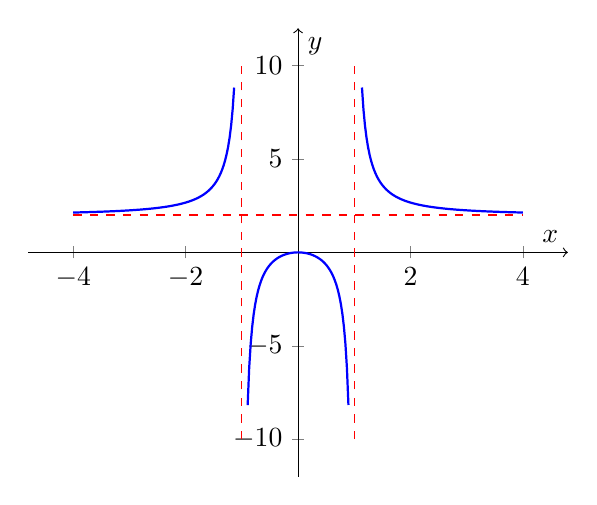
\begin{tikzpicture}
  \begin{axis}[
    axis lines = center,
    xlabel = $x$, ylabel = $y$,
    domain=-4:4,
    samples=300,
    ymin=-10, ymax=10,
    xmin=-4, xmax=4,
    restrict y to domain=-10:10,
    enlargelimits=true,
    legend pos=outer north east,
    axis line style={->},
    ]
    \addplot[blue, thick] {2*x^2/(x^2 - 1)};

    \draw[dashed, red] (axis cs:1,-10) -- (axis cs:1,10);
    \draw[dashed, red] (axis cs:-1,-10) -- (axis cs:-1,10);
    \draw[dashed, red] (axis cs:-4,2) -- (axis cs:4,2);

  \end{axis}
\end{tikzpicture}
\end{center}

\hfill

\noindent 6) Let $f(x) = x^4 +3x+1$. $f$ is continuous everywhere. IVT (Intermediate Value Theorem) states that $f$ takes any value on the interval $[a, b]$ between $f(a)$ and $f(b)$. Let us check $f(-1)$ and $f(-2)$.

\begin{equation*} f(-1) = (-1)^4 + 3(-1) + 1 = -1,\,\, f(-2) = (-2)^4 + 3(-2) + 1 = 11\end{equation*}

\hfill

\noindent By IVT, there exists at least one point on $[-2, -1]$ such that the value of $f$ is zero there. To show that this is the only point where $f(x) = 0$, we may use MVT (Mean Value Theorem). $f$ is differentiable on $(-2, -1)$ as well as it is continuous on $[-2, -1]$. By MVT, there exists a point $c$ such that

\begin{equation*} f'(c) = \frac{f(b) - f(a)}{b-a}\end{equation*} where $-2 \leq a \leq -1$ and $-2 \leq b \leq -1$. We can show that $f(x)$ has no more than one root on the interval $(-2, -1)$. Assume that we have $a$ and $b$ such that we have two distinct roots, meaning $f'(c) = 0$ somewhere on $(-2, -1)$. So,

\begin{equation*} f'(x) = 4x^3 + 3\,\rightarrow\,f'(c) = 4c^3+3\end{equation*}
\begin{equation*} f'(c) = 0\,\rightarrow\, 4c^3+3 = 0\,\rightarrow\,  c = \sqrt[3]{-\frac{3}{4}} > -1 \end{equation*}

\noindent The only point where $f(x) = 0$ is $c=\sqrt[3]{-\frac{3}{4}}$; however, it is outside the interval. For $x < \sqrt[3]{-\frac{3}{4}}$, the function is also strictly decreasing. This contradicts our assumption that we have two distinct roots on $(-2, -1)$. Therefore, there's only one root on the interval $(-2, -1)$.

\end{document}